\documentclass[10pt,letterpaper]{article}

\usepackage{cogsci}
\usepackage{pslatex}
\usepackage{apacite}
\usepackage{graphicx}

\title{Memory Driven Temporal Preparation: A Cognitive Model}
 
\author{{\large \bf Steven Bosch (s1861948)} \\
  Faculty of Mathematics and Natural Sciences}


\begin{document}
\maketitle

\begin{abstract}
Blabla

\textbf{Keywords:} 
temporal preparation; cue target interval timing; Hazard function; long term memory
\end{abstract}

\section{Introduction}
The human brain has many traits that we are hardly aware of during our everyday lives, even though these traits have a great impact on our experiences and actions. One such trait is the ability of cue target interval timing. Both consciously and unconsciously this ability is exercised in numerous situations, such as waiting for traffic lights, expecting a sound when something falls or simply expecting the second hand of a clock to move to the next second. What are the cognitive mechanisms behind this ability?

One theory encompasses the \textit{Hazard function}. This function describes that the conditional probability of the occurrence of a target event after the presentation of a cue increases over time given that the event has not yet occurred. While this function has been successfully used to predict interval timing behaviour \cite{Nobre, Vangkilde}, it does not provide an explanation as to the cognitive processes behind it. Moreover it does not take into account memory traces of preceding timing experiences. The past years research began on this basis \cite{Los1, Howard, Taatgen}. Los et al. (2014) developed what they called the \textit{multiple trace theory of temporal preparation} (MTP), in which every new trial causes a memory trace to be created, storing a temporal profile of that trial.This memory trace subsequently contributes to the preparation of subsequent trials. 

A recent experiment by Los et al. indicated that temporal preparation is indeed driven by memory \cite{Los2}. In the experiment different groups of participants were presented with different distributions of foreperiods between temporal cues and target stimuli. Three of these expimerents showed a transfer effect of this manipuation in a test phase where all participants received the same uniform distribution, indicating memory influence. 

In the present study this experiment was replicated. This paper discusses both the method and results of this replicate experiment, and a cognitive model that tries to capture the underlying cognitive processes, while producing similar test results.

\section{Experiment}
\subsection{Method}
In their experiment, Los et al. (2015)
\subsection{Results}

\section{Model}
\subsection{Method}
\subsection{Results}

\begin{figure}
	\centering
	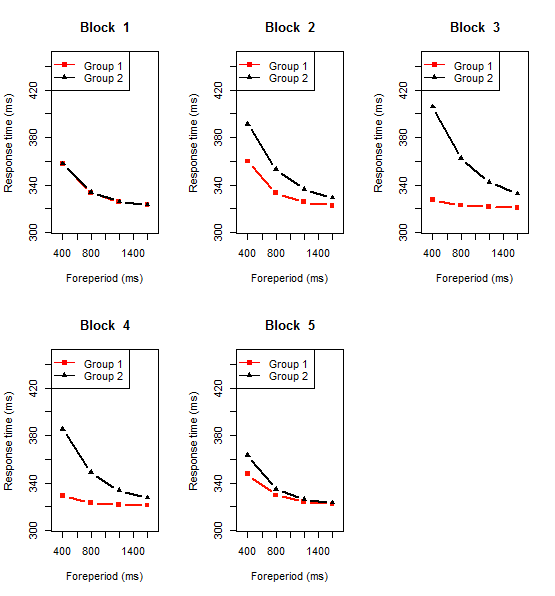
\includegraphics[width=\columnwidth]{5blocks2.png}
	\caption{Model results for two groups of `subjects' getting either exponential or anti-exponential distributions in their second and third block.}
	\label{5blocks}
\end{figure}

\section{Discussion}



\bibliographystyle{apacite}
\setlength{\bibleftmargin}{.125in}
\setlength{\bibindent}{-\bibleftmargin}
\bibliography{bibliography}

\end{document}
